\section{Discriminant Output Plots}
\label{Channel}

\vspace{0.1in}
\begin{center}
MATRIX ELEMENT OUTPUTS FOR THE ELECTRON CHANNEL WITH TWO JETS
\end{center}

\begin{figure}[!h!tbp]
\includegraphics[width=0.40\textwidth]
{figures/output/electron_2_1/All_tb_Discriminant}
\includegraphics[width=0.40\textwidth]
{figures/output/electron_2_1/All_tb_Discriminant_Zoom}
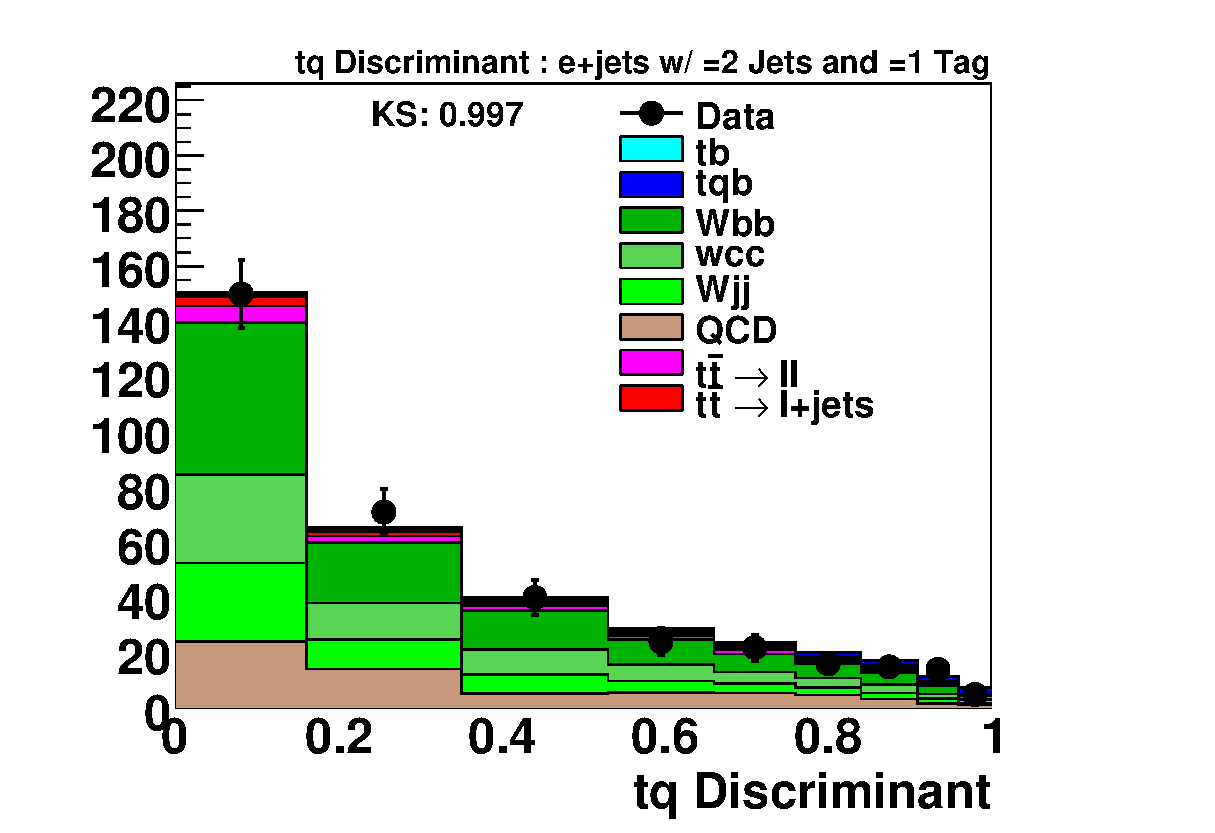
\includegraphics[width=0.40\textwidth]
{figures/output/electron_2_1/All_tq_Discriminant}
\includegraphics[width=0.40\textwidth]
{figures/output/electron_2_1/All_tq_Discriminant_Zoom}
\vspace{-0.1in}
\caption[e21]{Discriminant plots for the electron channel with one
$b$~tag. Upper row: $tb$ discriminant, lower row: $tq$ discriminant.
Left column, full discriminant range, right column, close-up of the high end of the distribution.}
\label{e_2_1}
\end{figure}

\begin{figure}[!h!tbp]
\includegraphics[width=0.40\textwidth]
{figures/output/electron_2_2/All_tb_Discriminant}
\includegraphics[width=0.40\textwidth]
{figures/output/electron_2_2/All_tb_Discriminant_Zoom}
\includegraphics[width=0.40\textwidth]
{figures/output/electron_2_2/All_tq_Discriminant}
\includegraphics[width=0.40\textwidth]
{figures/output/electron_2_2/All_tq_Discriminant_Zoom}
\vspace{-0.1in}
\caption[e22]{Discriminant plots for the electron channel with two
$b$~tags. The plot layout is the same as in Fig.~\ref{e_2_1}.}
\label{e_2_2}
\end{figure}

\clearpage

\begin{center}
MATRIX ELEMENT OUTPUTS FOR THE MUON CHANNEL WITH TWO JETS
\end{center}

\begin{figure}[!h!tbp]
\includegraphics[width=0.40\textwidth]
{figures/output/muon_2_1/All_tb_Discriminant}
\includegraphics[width=0.40\textwidth]
{figures/output/muon_2_1/All_tb_Discriminant_Zoom}
\includegraphics[width=0.40\textwidth]
{figures/output/muon_2_1/All_tq_Discriminant}
\includegraphics[width=0.40\textwidth]
{figures/output/muon_2_1/All_tq_Discriminant_Zoom}
\vspace{-0.1in}
\caption[e21]{Discriminant plots for the muon channel with one
$b$~tag. Upper row: $tb$ discriminant, lower row: $tq$ discriminant.
Left column, full discriminant range, right column, close-up of the high end of the distribution.}
\label{m_2_1}
\end{figure}

\begin{figure}[!h!tbp]
\includegraphics[width=0.40\textwidth]
{figures/output/muon_2_2/All_tb_Discriminant}
\includegraphics[width=0.40\textwidth]
{figures/output/muon_2_2/All_tb_Discriminant_Zoom}
\includegraphics[width=0.40\textwidth]
{figures/output/muon_2_2/All_tq_Discriminant}
\includegraphics[width=0.40\textwidth]
{figures/output/muon_2_2/All_tq_Discriminant_Zoom}
\vspace{-0.1in}
\caption[e22]{Discriminant plots for the muon channel with two
$b$~tags. The plot layout is the same as in Fig.~\ref{e_2_1}.}
\label{m_2_2}
\end{figure}

\clearpage

\vspace{0.1in}
\begin{center}
MATRIX ELEMENT OUTPUTS FOR THE ELECTRON CHANNEL WITH THREE JETS
\end{center}

\begin{figure}[!h!tbp]
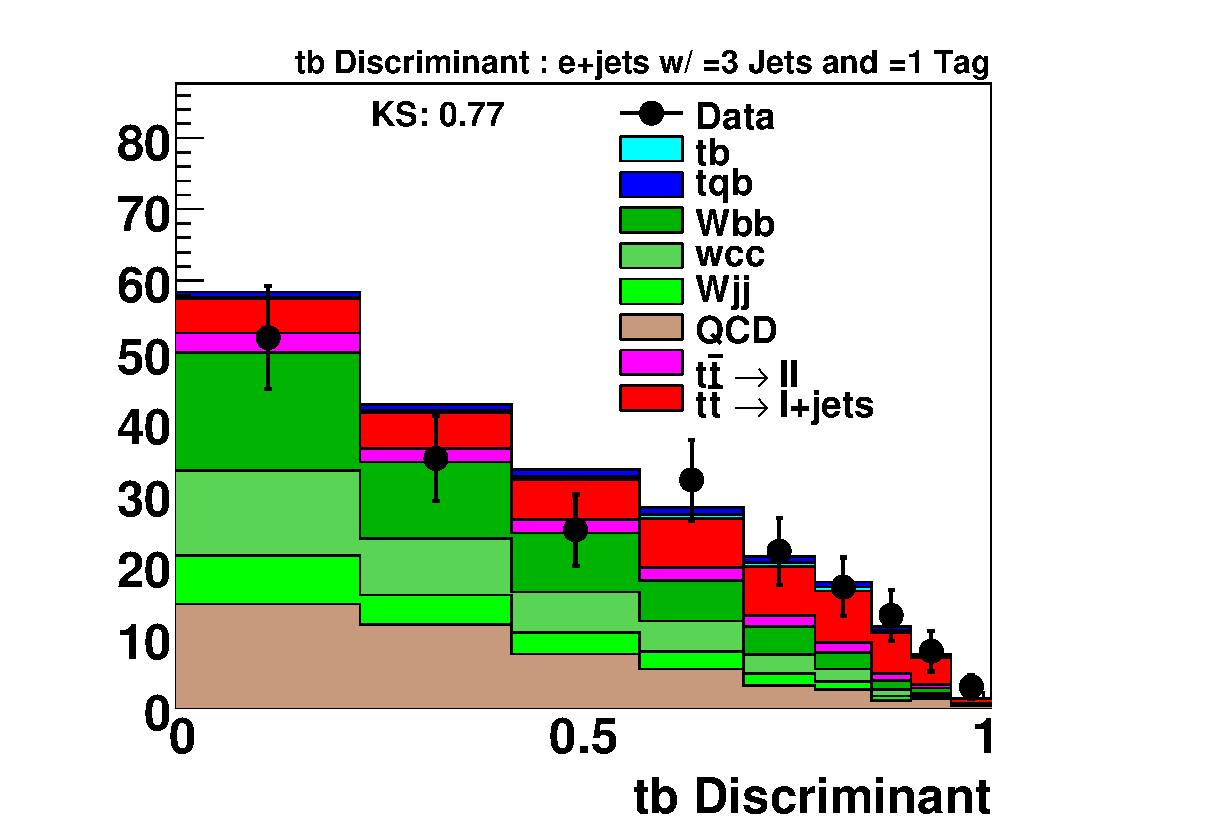
\includegraphics[width=0.40\textwidth]
{figures/output/electron_3_1/All_tb_Discriminant}
\includegraphics[width=0.40\textwidth]
{figures/output/electron_3_1/All_tb_Discriminant_Zoom}
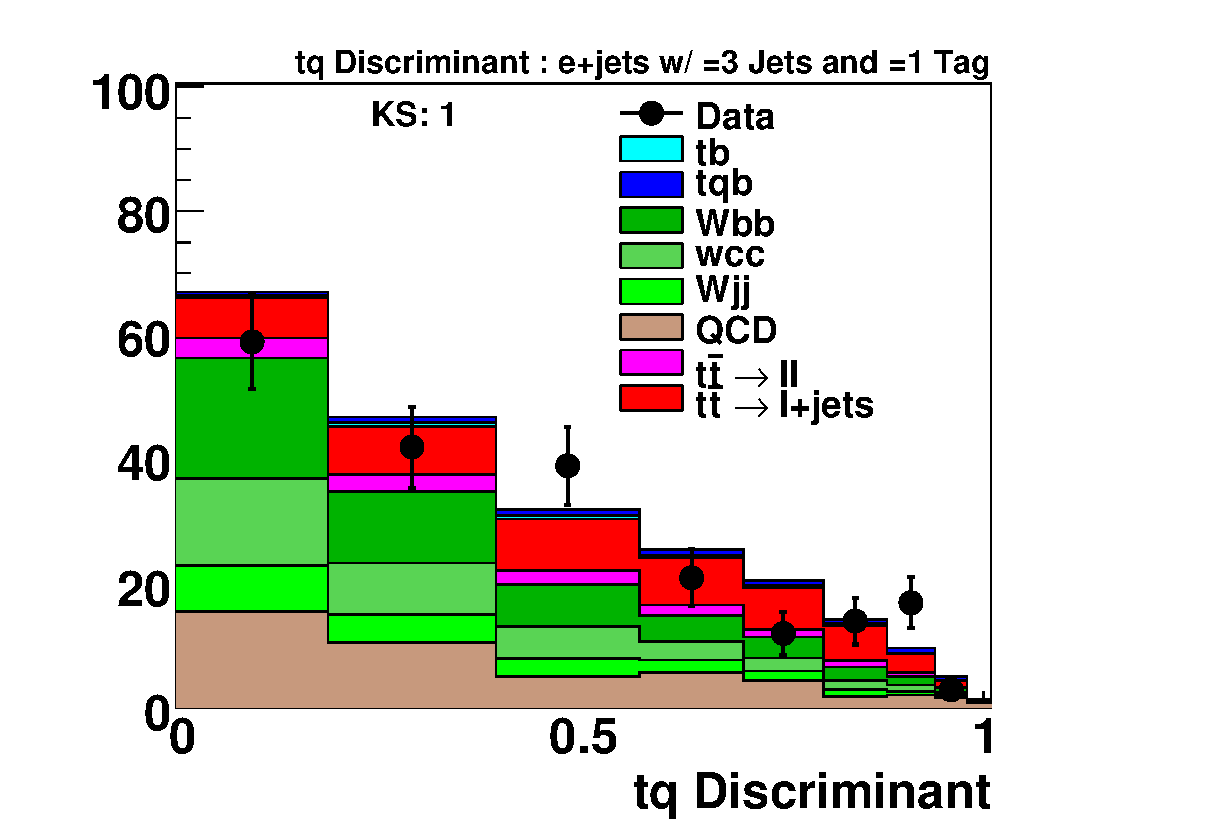
\includegraphics[width=0.40\textwidth]
{figures/output/electron_3_1/All_tq_Discriminant}
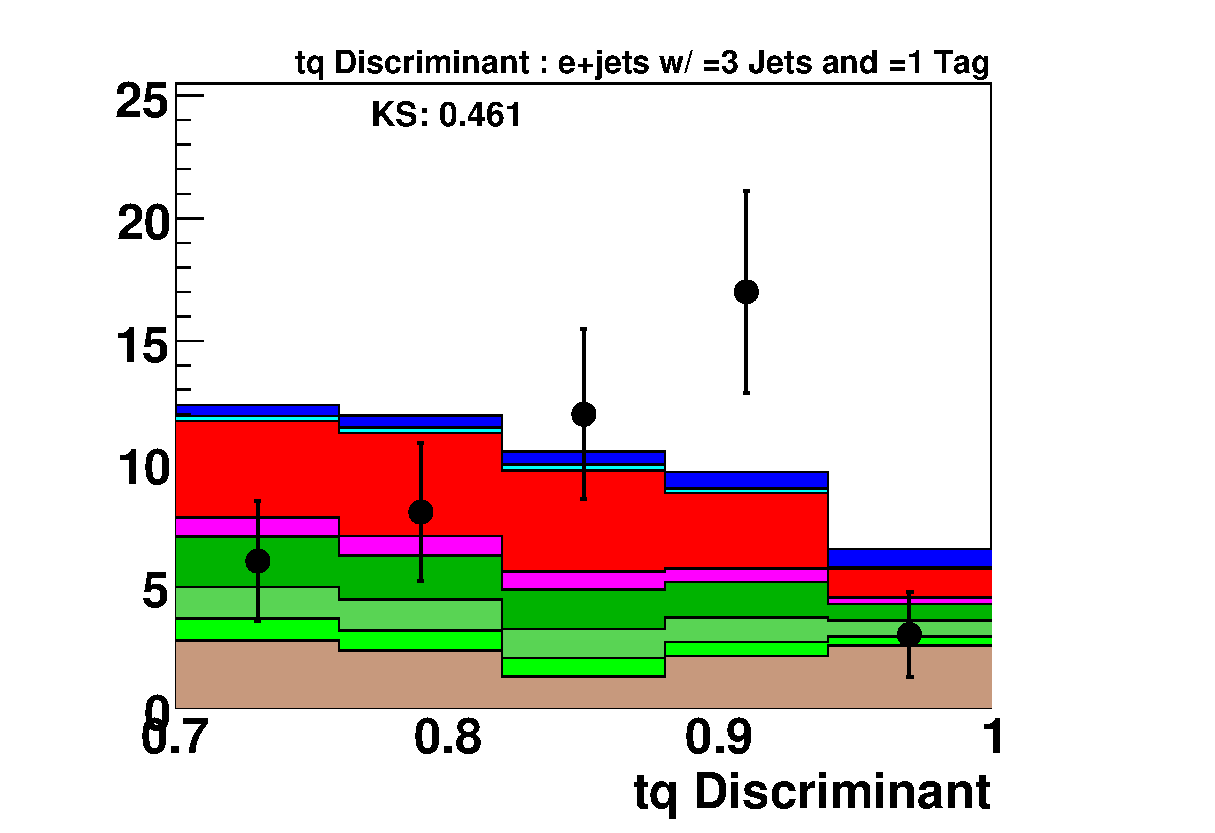
\includegraphics[width=0.40\textwidth]
{figures/output/electron_3_1/All_tq_Discriminant_Zoom}
\vspace{-0.1in}
\caption[e21]{Discriminant plots for the electron channel with one
$b$~tag. Upper row: $tb$ discriminant, lower row: $tq$ discriminant.
Left column, full discriminant range, right column, close-up of the high end of the distribution.}
\label{e_3_1}
\end{figure}

\begin{figure}[!h!tbp]
\includegraphics[width=0.40\textwidth]
{figures/output/electron_3_2/All_tb_Discriminant}
\includegraphics[width=0.40\textwidth]
{figures/output/electron_3_2/All_tb_Discriminant_Zoom}
\includegraphics[width=0.40\textwidth]
{figures/output/electron_3_2/All_tq_Discriminant}
\includegraphics[width=0.40\textwidth]
{figures/output/electron_3_2/All_tq_Discriminant_Zoom}
\vspace{-0.1in}
\caption[e22]{Discriminant plots for the electron channel with two
$b$~tags. The plot layout is the same as in Fig.~\ref{e_2_1}.}
\label{e_3_2}
\end{figure}

\clearpage

\begin{center}
MATRIX ELEMENT OUTPUTS FOR THE MUON CHANNEL WITH THREE JETS
\end{center}

\begin{figure}[!h!tbp]
\includegraphics[width=0.40\textwidth]
{figures/output/muon_3_1/All_tb_Discriminant}
\includegraphics[width=0.40\textwidth]
{figures/output/muon_3_1/All_tb_Discriminant_Zoom}
\includegraphics[width=0.40\textwidth]
{figures/output/muon_3_1/All_tq_Discriminant}
\includegraphics[width=0.40\textwidth]
{figures/output/muon_3_1/All_tq_Discriminant_Zoom}
\vspace{-0.1in}
\caption[e21]{Discriminant plots for the muon channel with one
$b$~tag. Upper row: $tb$ discriminant, lower row: $tq$ discriminant.
Left column, full discriminant range, right column, close-up of the high end of the distribution.}
\label{m_3_1}
\end{figure}

\begin{figure}[!h!tbp]
\includegraphics[width=0.40\textwidth]
{figures/output/muon_3_2/All_tb_Discriminant}
\includegraphics[width=0.40\textwidth]
{figures/output/muon_3_2/All_tb_Discriminant_Zoom}
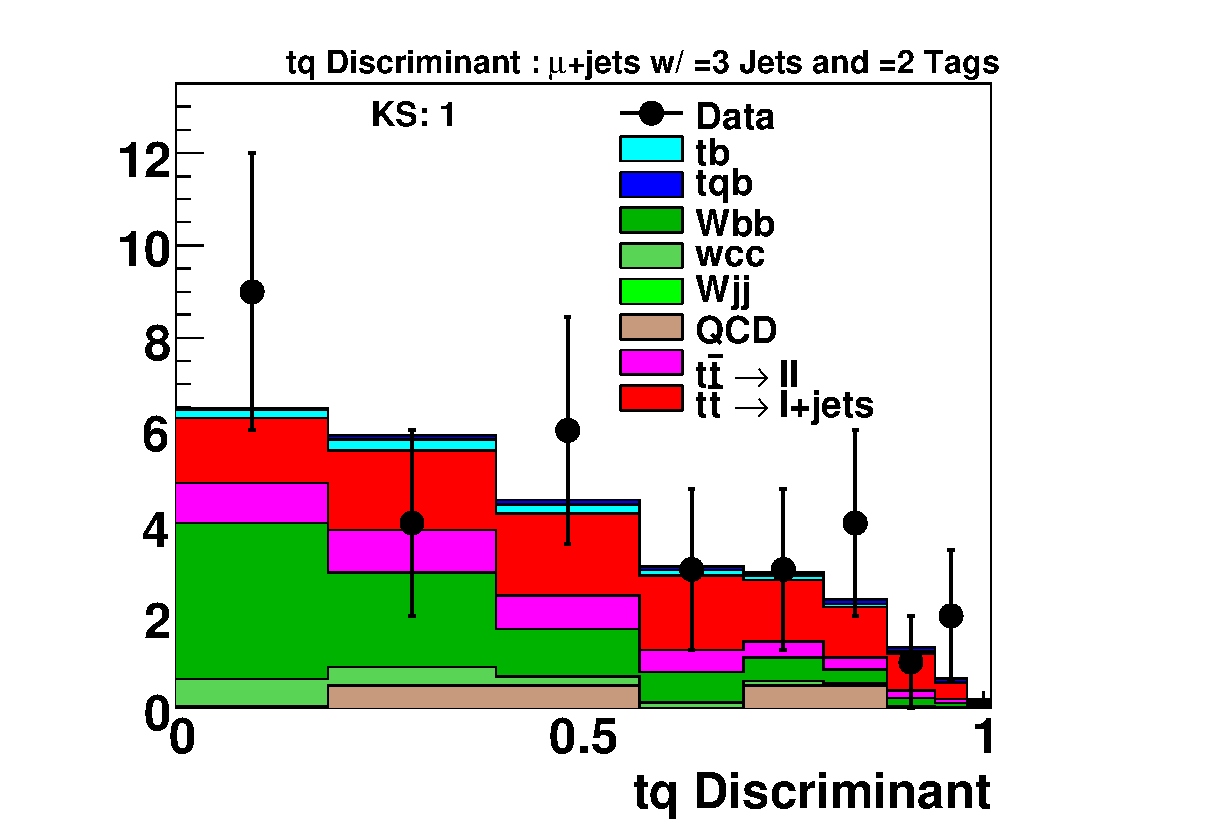
\includegraphics[width=0.40\textwidth]
{figures/output/muon_3_2/All_tq_Discriminant}
\includegraphics[width=0.40\textwidth]
{figures/output/muon_3_2/All_tq_Discriminant_Zoom}
\vspace{-0.1in}
\caption[e22]{Discriminant plots for the muon channel with two
$b$~tags. The plot layout is the same as in Fig.~\ref{e_2_1}.}
\label{m_3_2}
\end{figure}





